\documentclass{vkr}
\usepackage[english, russian]{babel} % переносы
\usepackage{graphicx} % для вставки картинок
\graphicspath{{images/}} % путь к изображениям
\usepackage[hidelinks]{hyperref}
\usepackage{float} % определяет метод H для рисунка с переносом на следующую страницу, ели не помещается
\usepackage{pdflscape}
\addto{\captionsrussian}{\renewcommand{\refname}{СПИСОК ИСПОЛЬЗОВАННЫХ ИСТОЧНИКОВ}}
\usepackage{xltabular} % для вставки таблиц
\usepackage{makecell}
\renewcommand\theadfont{} % шрифт в /thead
\usepackage{array} % для определения новых типов столбцов таблиц
\newcolumntype{T}{>{\centering\arraybackslash}X} % новый тип столбца T - автоматическая ширина столбца с выравниванием по центру
\newcolumntype{R}{>{\raggedleft\arraybackslash}X} % новый тип столбца R - автоматическая ширина столбца с выравниванием по правому краю
\newcolumntype{C}[1]{>{\centering\let\newline\\\arraybackslash\hspace{0pt}}m{#1}} % новый тип столбца C - фиксированная ширина столбца с выравниванием по центру
\newcolumntype{r}[1]{>{\raggedleft\arraybackslash}p{#1}} % новый тип столбца r - фиксированная ширина столбца с выравниванием по правому краю
\newcommand{\centrow}{\centering\arraybackslash} % командой \centrow можно центрировать одну ячейку (заголовок) в столбце типа X или p, оставив в оcтальных ячейках другой тип выравнивания
\newcommand{\finishhead}{\endhead\hline\endlastfoot}
\newcommand{\continuecaption}[1]{\caption*{#1}\\ \hline }
\usepackage{etoolbox}
\AtBeginEnvironment{xltabular}{\refstepcounter{tablecnt}} % подсчет таблиц xltabular, обычные таблицы подсчитываются в классе

\usepackage[tableposition=top]{caption} % подпись таблицы вверху
\captionsetup{strut=off}
\setlength{\intextsep}{0pt} % Vertical space above & below [h] floats
\setlength{\textfloatsep}{0pt} % Vertical space below (above) [t] ([b]) floats
\DeclareCaptionLabelFormat{gostfigure}{Рисунок #2} %подпись рисунка
\DeclareCaptionLabelFormat{gosttable}{Таблица #2} %подпись таблицы
\DeclareCaptionLabelSeparator{gost}{~--~} %разделитель в рисунках и таблицах
\captionsetup{labelsep=gost}
\captionsetup[figure]{aboveskip=10pt,belowskip=4mm,justification=centering,labelformat=gostfigure} % настройка подписи рисунка
\captionsetup[table]{font={stretch=1.41},skip=0pt,belowskip=0pt,aboveskip=8.5pt,singlelinecheck=off,labelformat=gosttable} % настройка подписи таблицы

\setlength{\LTpre}{8mm} % отступ сверху таблицы
\setlength{\LTpost}{6mm} % отступ снизу таблицы

\usepackage{enumitem}
\setlist{nolistsep,wide=\parindent,itemindent=*} % отступы вокруг списков, выравнивание с учетом разделителя

\usepackage{color} %% это для отображения цвета в коде
\usepackage{listings} %% листинги кода
\setmonofont[Scale=0.7]{Verdana} % моноширный шрифт для листинга

\definecolor{codegreen}{rgb}{0,0.6,0}
\definecolor{codegray}{rgb}{0.5,0.5,0.5}
\definecolor{codepurple}{rgb}{0.58,0,0.82}

\lstset{ %
	language=C,                 % выбор языка для подсветки (здесь это С)
	numbers=left,               % где поставить нумерацию строк (слева\справа)
	numberstyle=\tiny,           % размер шрифта для номеров строк
	stepnumber=1,                   % размер шага между двумя номерами строк
	numbersep=5pt,                % как далеко отстоят номера строк от подсвечиваемого кода
	commentstyle=\color{codegreen},
	keywordstyle=\color{magenta},
	numberstyle=\tiny\color{codegray},
	stringstyle=\color{codepurple},
	basicstyle=\linespread{0.95}\ttfamily,
	backgroundcolor=\color{white}, % цвет фона подсветки - используем \usepackage{color}
	showspaces=false,            % показывать или нет пробелы специальными отступами
	showstringspaces=false,      % показывать или нет пробелы в строках
	showtabs=false,             % показывать или нет табуляцию в строках
	frame=single,              % рисовать рамку вокруг кода
	tabsize=2,                 % размер табуляции по умолчанию равен 2 пробелам
	captionpos=t,              % позиция заголовка вверху [t] или внизу [b] 
	breaklines=true,           % автоматически переносить строки (да\нет)
	breakatwhitespace=false, % переносить строки только если есть пробел
	escapeinside={\%*}{*)}   % если нужно добавить комментарии в коде
}

\makeatletter % чтобы допускались русские комментарии в листингах
\lst@InputCatcodes
\def\lst@DefEC{%
	\lst@CCECUse \lst@ProcessLetter
	^^80^^81^^82^^83^^84^^85^^86^^87^^88^^89^^8a^^8b^^8c^^8d^^8e^^8f%
	^^90^^91^^92^^93^^94^^95^^96^^97^^98^^99^^9a^^9b^^9c^^9d^^9e^^9f%
	^^a0^^a1^^a2^^a3^^a4^^a5^^a6^^a7^^a8^^a9^^aa^^ab^^ac^^ad^^ae^^af%
	^^b0^^b1^^b2^^b3^^b4^^b5^^b6^^b7^^b8^^b9^^ba^^bb^^bc^^bd^^be^^bf%
	^^c0^^c1^^c2^^c3^^c4^^c5^^c6^^c7^^c8^^c9^^ca^^cb^^cc^^cd^^ce^^cf%
	^^d0^^d1^^d2^^d3^^d4^^d5^^d6^^d7^^d8^^d9^^da^^db^^dc^^dd^^de^^df%
	^^e0^^e1^^e2^^e3^^e4^^e5^^e6^^e7^^e8^^e9^^ea^^eb^^ec^^ed^^ee^^ef%
	^^f0^^f1^^f2^^f3^^f4^^f5^^f6^^f7^^f8^^f9^^fa^^fb^^fc^^fd^^fe^^ff%
	^^^^20ac^^^^0153^^^^0152%
	% Basic Cyrillic alphabet coverage
	^^^^0410^^^^0411^^^^0412^^^^0413^^^^0414^^^^0415^^^^0416^^^^0417%
	^^^^0418^^^^0419^^^^041a^^^^041b^^^^041c^^^^041d^^^^041e^^^^041f%
	^^^^0420^^^^0421^^^^0422^^^^0423^^^^0424^^^^0425^^^^0426^^^^0427%
	^^^^0428^^^^0429^^^^042a^^^^042b^^^^042c^^^^042d^^^^042e^^^^042f%
	^^^^0430^^^^0431^^^^0432^^^^0433^^^^0434^^^^0435^^^^0436^^^^0437%
	^^^^0438^^^^0439^^^^043a^^^^043b^^^^043c^^^^043d^^^^043e^^^^043f%
	^^^^0440^^^^0441^^^^0442^^^^0443^^^^0444^^^^0445^^^^0446^^^^0447%
	^^^^0448^^^^0449^^^^044a^^^^044b^^^^044c^^^^044d^^^^044e^^^^044f%
	^^^^0401^^^^0451%
	%%%
	^^00}
\lst@RestoreCatcodes
\makeatother

% Режим шаблона (должен быть включен один из трех)
%\ВКРtrue
%\Практикаtrue
\Курсоваяtrue

\newcommand{\Дисциплина}{<<Проектирование и архитектура программных систем>>} % для курсовой
\newcommand{\КодСпециальности}{09.03.04} % Курсовая
\newcommand{\Специальность}{Программная инженерия} % Курсовая
\newcommand{\Тема}{Aлгоритмическая библиотека} % ВКР Курсовая
\newcommand{\ГдеПроводитсяПрактика}{Юго-Западном государственном университете} % для практики
\newcommand{\РуководительПрактПредпр}{Куркина А. В.} % для практики
\newcommand{\ДолжнРуководительПрактПредпр}{директор} % для практики
\newcommand{\РуководительПрактУнивер}{Чаплыгин А. А.} % для практики
\newcommand{\ДолжнРуководительПрактУнивер}{к.т.н. доцент} % для практики
\newcommand{\Автор}{Рефуз  К. Б.}
\newcommand{\АвторРод}{Рефуз  К. Б.}
\newcommand{\АвторПолностьюРод}{Иванова Ивана Ивановича} % для практики
\newcommand{\Шифр}{21-06-0377}
\newcommand{\Курс}{3} % для практики
\newcommand{\Группа}{ПО-12б}
\newcommand{\Руководитель}{А. А. Чаплыгин} % для ВКР и курсовой
\newcommand{\Нормоконтроль}{А. А. Чаплыгин} % для ВКР
\newcommand{\ЗавКаф}{А. В. Малышев} % для ВКР
\newcommand{\ДатаПриказа}{«07» апреля 2023~г.} % для ВКР
\newcommand{\НомерПриказа}{1505-с} % для ВКР
\newcommand{\СрокПредоставления}{«15» Март 2024~г.} % для ВКР, курсового

\begin{document}
\maketitle
\ifПрактика{}\else{
	\newpage
\begin{center}
	\large\textbf{Минобрнауки России}
	
	\large\textbf{Юго-Западный государственный университет}
	\vskip 1em
	\normalsize{Кафедра программной инженерии}
	\vskip 1em
	\ifВКР{
		\begin{flushright}
			\begin{tabular}{p{.4\textwidth}}
				\centrow УТВЕРЖДАЮ: \\
				\centrow Заведующий кафедрой \\
				\hrulefill \\
				\setarstrut{\footnotesize}
				\centrow\footnotesize{(подпись, инициалы, фамилия)}\\
				\restorearstrut
				«\underline{\hspace{1cm}}»
				\underline{\hspace{3cm}}
				20\underline{\hspace{1cm}} г.\\
			\end{tabular}
		\end{flushright}
	}\fi
\end{center}
\vspace{1em}
\begin{center}
	\large
	\ifВКР{
		ЗАДАНИЕ НА ВЫПУСКНУЮ КВАЛИФИКАЦИОННУЮ РАБОТУ
		ПО ПРОГРАММЕ БАКАЛАВРИАТА}
	\else
	ЗАДАНИЕ НА КУРСОВУЮ РАБОТУ (ПРОЕКТ)
	\fi
	\normalsize
\end{center}
\vspace{1em}
{\parindent0pt
	Студента \АвторРод, шифр\ \Шифр, группа \Группа
	
	1. Тема «\Тема\ \ТемаВтораяСтрока»
	\ifВКР{
		утверждена приказом ректора ЮЗГУ от \ДатаПриказа\ № \НомерПриказа
	}\fi.
	
	2. Срок предоставления работы к защите \СрокПредоставления
	
	3. Исходные данные для создания программной системы:
	
	3.1. Перечень решаемых задач:}

\renewcommand\labelenumi{\theenumi)}

\begin{enumerate}
	\item  разработка концептуальной модели алгоритмической библиотеки;
	\item разработать алгоритмическая библиотека;
	\item Составление и тестирование алгоритмических библиотек.
\end{enumerate}

{\parindent0pt
	3.2. Входные данные и требуемые результаты для программы:}

\begin{enumerate}
	\item Входными данными для программной системы являются: команды растрового редактора.
	\item Выходными данными для программной системы являются: фигуры, выводящиеся на окно приложения, .
\end{enumerate}

{\parindent0pt
	
	4. Содержание работы (по разделам):
	
	4.1. Введение
	
	4.1. Анализ предметной области
	
	4.2. Техническое задание: основание для разработки, назначение разработки,
	требования к программной системе, требования к оформлению документации.
	
	4.3. Технический проект: общие сведения о программной системе, проект
	данных программной системы, проектирование архитектуры программной системы, проектирование пользовательского интерфейса программной системы.
	
	4.4. Рабочий проект: спецификация компонентов и классов программной системы, тестирование программной системы, сборка компонентов программной системы.
	
	4.5. Заключение
	
	4.6. Список использованных источников
	
	5. Перечень графического материала:
	
	\списокПлакатов
	
	\vskip 2em
	\begin{tabular}{p{6.8cm}C{3.8cm}C{4.8cm}}
		Руководитель \ifВКР{ВКР}\else работы (проекта) \fi & \lhrulefill{\fill} & \fillcenter\Руководитель\\
		\setarstrut{\footnotesize}
		& \footnotesize{(подпись, дата)} & \footnotesize{(инициалы, фамилия)}\\
		\restorearstrut
		Задание принял к исполнению & \lhrulefill{\fill} & \fillcenter\Автор\\
		\setarstrut{\footnotesize}
		& \footnotesize{(подпись, дата)} & \footnotesize{(инициалы, фамилия)}\\
		\restorearstrut
	\end{tabular}
}

\renewcommand\labelenumi{\theenumi.}
	\abstract{РЕФЕРАТ}

Объем работы равен \formbytotal{lastpage}{страниц}{е}{ам}{ам}. Работа содержит \formbytotal{figurecnt}{иллюстраци}{ю}{и}{й}, \formbytotal{tablecnt}{таблиц}{у}{ы}{}, \arabic{bibcount} библиографических источников и \formbytotal{числоПлакатов}{лист}{}{а}{ов} графического материала. Количество приложений – 2. Графический материал представлен в приложении А. Фрагменты исходного кода представлены в приложении Б.

Перечень ключевых слов: алгоритм, администратор, пользовател, устаревшие методы, добавление, удаление, модификация.

Объектом разработки является редактор алгоритмической библиотеки, который позволяет пользователю искать различные предлагаемые алгоритмы в программе и позволяет администратору изменять добавлять и удалять алгоритм .

Целью проекта является создание удобной и функциональной алгоритмической библиотеки, облегчающей поиск алгоритмов

В процессе создания библиотека алгоритмов была создана с использованием современного языка программирования Python.

\selectlanguage{english}
\abstract{ABSTRACT}

The volume of work is \formbytotal{lastpage}{page}{}{s}{s}. The work contains \formbytotal{figurecnt}{illustration}{}{s}{s}, \formbytotal{tablecnt}{table}{}{s}{s}, \arabic{bibcount} bibliographic sources and \formbytotal{числоПлакатов}{sheet}{}{s}{s} of graphic material. The number of applications is 2. The graphic material is presented in annex A. The layout of the site, including the connection of components, is presented in annex B.

The list of keywords: algorithm, administrator, user, outdated methods, addition, delete, modification.

The object of the development is the editor of the algorithmic library, which allows the user to search for various proposed algorithms in the program and allows the administrator to change, add and delete the algorithm.

The aim of the project is to create a convenient and functional algorithmic library that facilitates the search for algorithms

During the creation process, the algorithm library was created using the modern Python programming language.
\selectlanguage{russian}}\fi
	\tableofcontents
\section*{ОБОЗНАЧЕНИЯ И СОКРАЩЕНИЯ}

БД -- база данных.

ИС -- информационная система.

ИТ -- информационные технологии. 

КТС -- комплекс технических средств.

ОМТС -- отдел материально-технического снабжения. 

ПО -- программное обеспечение.

РП -- рабочий проект.

СУБД -- система управления базами данных.

ТЗ -- техническое задание.

ТП -- технический проект.


\ifПрактика{}\else{\section*{ВВЕДЕНИЕ}
\addcontentsline{toc}{section}{ВВЕДЕНИЕ}
Библиотека алгоритмов - это набор предварительно написанных функций, классов или модулей, которые обеспечивают эффективные и готовые к использованию реализации обычно используемых алгоритмов.

Алгоритмические библиотеки сыграли решающую роль в развитии вычислительной техники и решении проблем. Первоначально появившиеся в 1950-х и 1960-х годах, эти библиотеки были разработаны для предоставления эффективных решений алгоритмических задач, возникавших при обработке данных на ранних компьютерах. Со временем эти библиотеки эволюционировали и теперь включают в себя широкий спектр алгоритмов, от классических алгоритмов сортировки до алгоритмов расширенного поиска, методов оптимизации и алгоритмов построения графиков.

В настоящее время существует множество графических редакторов. Они имеют различную стоимость и набор функций. Некоторые из них предназначены для профессиональной работы с изображениями, а другие - для обычных пользователей.

\emph{Цель данной работы} - разработка библиотеки алгоритмов. Для достижения этой цели необходимо решить \emph{следующие задачи:}
\begin{itemize}
	\item Провести анализ предметной области;
	\item Разработать концептуальную модель библиотеки алгоритмов;
	\item Реализовать библиотеку.
\end{itemize}

\emph{Структура и объем работы.} Отчет состоит из введения, 4 основных разделов, заключения, списка использованных источников и 2 приложений. Текст отчета о квалификации составляет \formbytotal{page}{страниц}{е}{ам}{ам}.

\emph{Во введении} сформулирована цель работы, определены задачи разработки, описана структура работы и представлен краткий обзор каждого из разделов.

\emph{В первом разделе} на этапе описания технических характеристик предметной области собирается информация о существующих библиотеках алгоритмов.

\emph{Во втором разделе} на этапе составления технического задания устанавливаются требования к разрабатываемой библиотеке алгоритмов.

\emph{В третьем разделе} на этапе технического проектирования представлены проектные решения для библиотеки алгоритмов.

\emph{В четвертом разделе} представлен список классов и их методов, использованных при разработке библиотеки алгоритмов, а также проведено тестирование разработанной библиотеки.

В заключении изложены основные результаты работы, полученные в процессе разработки.

В приложении А представлен графический материал.
В приложении Б представлены фрагменты исходного кода.





}\fi
\section{Анализ предметной области}
\subsection{История развития алгоритмических библиотек}

История разработки алгоритмических библиотек восходит к ранним дням информатики и программирования. В первые десятилетия развития информатики программы часто писались для конкретных задач, а алгоритмы часто встраивались непосредственно в код этих программ. Однако с ростом сложности программного обеспечения и компьютерных систем становилось все более очевидным, что для эффективного управления алгоритмами необходим модульный и многоразовый подход.

В 1950-х и 1960-х годах, когда информатика начала выделяться в отдельную академическую область, начали разрабатываться первые алгоритмические библиотеки. Эти ранние библиотеки часто были специфичны для конкретной платформы или языка программирования и в основном использовались в рамках исследований и разработок в университетах и исследовательских лабораториях.

В течение следующих десятилетий, с расширением компьютерной индустрии и появлением языков программирования, алгоритмические библиотеки росли в геометрической прогрессии. Стандартизированные и обобщенные библиотеки были разработаны для широкого спектра областей, от математики и информатики до практических приложений, таких как манипулирование строками символов, сжатие данных и криптография.

В 1980-х и 1990-х годах, с появлением интернета и появлением программного обеспечения с открытым исходным кодом, многие алгоритмические библиотеки были разработаны и распространены как бесплатное программное обеспечение. 

Сегодня алгоритмические библиотеки являются неотъемлемой частью инструментария любого программиста или разработчика программного обеспечения. Они используются во множестве приложений, от простых алгоритмов сортировки до передовых методов машинного обучения и искусственного интеллекта. 

\section{Техническое задание}
\subsection{Основание для разработки}

Основанием для разработки является потребность в создании растрового редактора в рамках проекта по предмету "Проектирование и разработка программных систем".

\subsection{Цель и назначение разработки}

Основная цель этого проекта-разработать алгоритмические библиотеки enn используя технологии Python.

Цель разработки алгоритмической библиотеки - объединить простой и сложный лагорифмический поиск.

Задачи данной разработки включают:

\emph{для пользователя:}
\begin{itemize}
	\item используется для поиска алгоритма.
	\item позволяет отображать содержимое поляризатора.
\end{itemize}
\emph{для администратора:}
\begin{itemize}
	\item позволяет изменить режим пропуска администратора.
	\item позволяет изменять алгоритм.
	\item позволяет добавить алгоритм.
	\item используется для подавления алгоритма.
\end{itemize}

\subsection{Описание алгоритмической библиотеки}

Библиотека алгоритмов представляет собой программное обеспечение, разработанное для организации и управления набором алгоритмов. Она обладает следующими особенностями:
\begin{enumerate}
	\item \textbf{Навигация:} Доступен боковой панельный список всех алгоритмов с возможностью прокрутки, обеспечивая удобную навигацию между доступными вариантами.
	
	\item \textbf{Отображение содержимого:} Для выбранного алгоритма предоставляется область текста, где отображается его содержание с подробным описанием и примерами использования, что помогает пользователям понять его работу.
	
	\item \textbf{Режимы доступа:} Реализованы два режима доступа - пользовательский и администраторский, с обеспечением безопасности через аутентификацию по паролю для режима администратора.
	
	\item \textbf{Редактирование и управление:} Администраторы имеют возможность добавлять, редактировать и удалять алгоритмы, а также изменять пароль администратора для обеспечения полного контроля над библиотекой алгоритмов.

	
	\subsubsection{Функциональные элементы}
	Интерфейс должен предоставлять следующие элементы и функции:
	\begin{itemize}
	\item \textbf{Выбор инструментов:} Пользователи должны иметь возможность выбирать необходимые инструменты из специальной панели, обеспечивая таким образом простой и интуитивный выбор функций библиотеки.
	
	\item \textbf{Создание алгоритмов:} Должна быть возможность создавать новые алгоритмы и определять их характеристики с помощью специальных инструментов, позволяя пользователям вносить свой вклад в содержание библиотеки.
	
	\item \textbf{Редактирование алгоритмов:} Пользователи должны иметь возможность изменять существующие алгоритмы, настраивая их параметры или добавляя дополнительные функции, чтобы соответствовать их конкретным потребностям.
	
	\item \textbf{Удаление алгоритмов:} Должна быть возможность удаления нежелательных алгоритмов из библиотеки, предоставляя пользователям полный контроль над ее содержимым и качеством.
	
	\end{itemize}
	
	
	
	Композиция интерфейса редактора представлена на рисунке 2.1  и 2.2. 
	
	\begin{figure}[H]
		\centering
		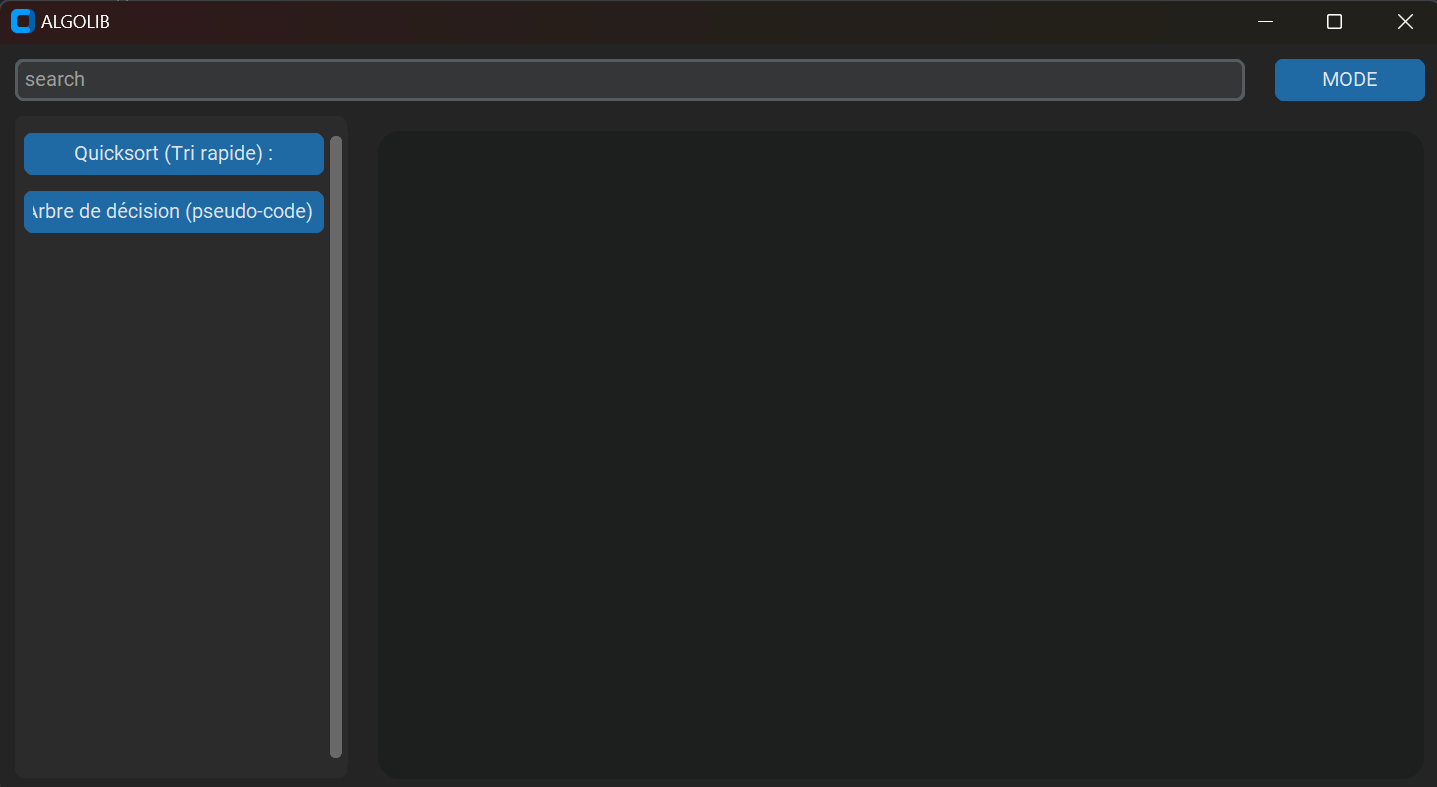
\includegraphics[width=0.7\linewidth]{images/macpaint}
		\caption{Компоновка графического интерфейса алгоритмической библиотеки.}
		\label{fig:redac_comp}
	\end{figure}

	\begin{figure}[H]
		\centering
		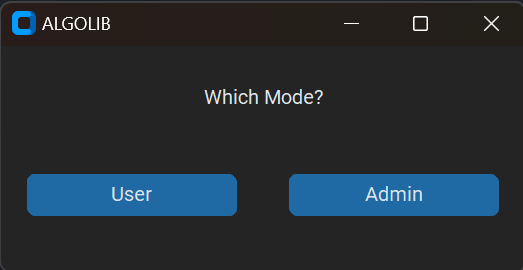
\includegraphics[width=0.7\linewidth]{images/paint}
		\caption{интерфейс с выбором из двух доступных режимов}
		\label{fig:redac_comp}
	\end{figure}
	\newpage
	
	
	
	
	
	\subsection{Требования пользователя к интерфейсу алгоритмической библиотеки}
	
	Ралгоритмическая библиотека должна создать простой и удобный интерфейс и предоставить следующие функции:
	\begin{itemize}
	\item бар поиска для фильтрации результатов по названию алгоритма.
	\item левая боковая панель с раскрывающимся списком всех алгоритмов.
	\item текстовая область с правой стороны для отображения содержимого выбранного алгоритма.
	\end{itemize}
	
	%\begin{figure}[ht]
	%\caption{Композиция шаблона сайта}
	%\label{templ:image}
	%\end{figure}
	%\vspace{-\figureaboveskip} % двойной отступ не нужен (можно использовать, если раздел заканчивается картинкой)
	
	\subsection{Моделирование вариантов использования}
	\subsubsection{Диаграмма прецедентов}
	Для библиотеки алгоритмов было разработано моделирование, позволяющее четко визуализировать различные варианты использования этой библиотеки. Это моделирование облегчает физическую разработку и подробный анализ взаимодействий между различными функциями и компонентами библиотеки. При создании этого моделирования предпочтение было отдано использованию языка визуального моделирования UML.
	
	Диаграмма вариантов использования описывает основную функциональность библиотеки алгоритмов. Это включает в себя действия, которые библиотека будет выполнять при ее использовании. Диаграмма представляет систему в виде серии вариантов использования, которые предлагаются пользователям или объектам, взаимодействующим с библиотекой. Вариант использования описывает набор действий, которые пользователь может выполнять с помощью библиотеки алгоритмов.
	
	На основе анализа функциональной области библиотеки алгоритмов необходимо реализовать следующие варианты использования :
	
	\begin{enumerate}
	\item  Поиск алгоритмов по названию.
	\item Просмотр подробной информации о конкретном алгоритме, включая его описание.
	\item Добавление новых алгоритмов в библиотеку или изменение существующих.
	\item Удаление алгоритмов из библиотеки.
	\item Обновление информации о библиотеке и ее содержимом.
	\item Изменение пароля администратора.
	\end{enumerate}
	
	
	
	\begin{figure}[ht]
		\center{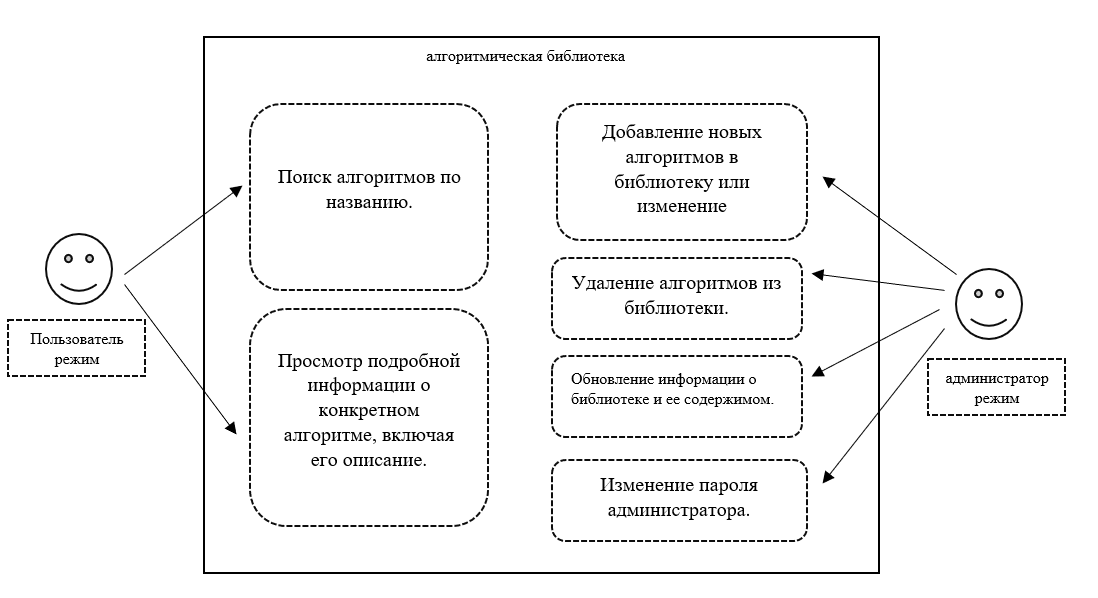
\includegraphics[width=1\linewidth]{precedent}}
		\caption{Диаграмма прецедентов}
		\label{precend:image}
	\end{figure}
	
	\subsubsection{Сценарии прецедентов программы}
	
	\begin{enumerate}
		\item Сценарий для случая использования "Поиск алгоритма":
		\begin{itemize}
			\item Основной исполнитель: Пользователь;
			\item Заинтересованные стороны и их требования: Пользователь вводит название алгоритма в строку поиска;
			\item Предварительное условие: Пользователь авторизован;
			\item Основной успешный сценарий: Алгоритм автоматически сортируется при вводе пользователем.
		\end{itemize}
		
		\item Сценарий для случая использования "Показать описание выбранного алгоритма":
		\begin{itemize}
			\item Основной исполнитель: Пользователь;
			\item Заинтересованные стороны и их требования: Пользователь должен выбрать алгоритм и отобразить его описание;
			\item Предварительное условие: Пользователь открыл библиотеку алгоритмов;
			\item Основной успешный сценарий: Пользователь нажимает на соответствующую кнопку для выбора желаемого алгоритма и отображения его описания.
		\end{itemize}
		
		\item Сценарий для случая использования "Добавить новый алгоритм":
		\begin{itemize}
			\item Основной исполнитель: Администратор;
			\item Заинтересованные стороны и их требования: Администратор должен добавить новый алгоритм в библиотеку;
			\item Предварительное условие: Администратор авторизован как администратор;
			\item Основной успешный сценарий: Администратор нажимает на кнопку "Добавить алгоритм" и следует инструкциям для успешного добавления алгоритма.
		\end{itemize}
		
		\item Сценарий для случая использования "Удалить алгоритм":
		\begin{itemize}
			\item Основной исполнитель: Администратор;
			\item Заинтересованные стороны и их требования: Администратор должен удалить существующий алгоритм из библиотеки;
			\item Предварительное условие: Администратор авторизован как администратор;
			\item Основной успешный сценарий: Администратор нажимает на кнопку "Удалить алгоритм" и следует инструкциям для успешного удаления алгоритма.
		\end{itemize}
		
		\item Сценарий для случая использования "Изменить алгоритм":
		\begin{itemize}
			\item Основной исполнитель: Администратор;
			\item Заинтересованные стороны и их требования: Администратор должен изменить существующий алгоритм в библиотеке;
			\item Предварительное условие: Администратор авторизован как администратор;
			\item Основной успешный сценарий: Администратор нажимает на кнопку "Изменить алгоритм" и следует инструкциям для успешного изменения алгоритма.
		\end{itemize}
		
		\item Сценарий для случая использования "Изменить пароль":
		\begin{itemize}
			\item Основной исполнитель: Администратор;
			\item Заинтересованные стороны и их требования: Администратор должен изменить свой пароль;
			\item Предварительное условие: Администратор авторизован как администратор;
			\item Основной успешный сценарий: Администратор нажимает на кнопку "Изменить пароль" и следует инструкциям для успешного изменения пароля.
		\end{itemize}
	\end{enumerate}
	
	\subsection{Требования к оформлению документации}
	
	Разработка программной документации и программного изделия должна производиться согласно ГОСТ 19.102-77 и ГОСТ 34.601-90. Единая система программной документации.
	
\section{Технический проект}
\subsection{Общая характеристика организации решения задачи}
Вы должны спроектировать и разработать алгоритмическую библиотеку. библиотека реализована на Python.

\subsection{Описание используемых библеотек и языков программирования}
Проект реализован с использованием языка Python.


\subsection{Технические детали проекта}
\subsubsection{Интерфейс редактора}
Интерфейс библиотеки алгоритмов состоит из панели поиска для фильтрации результатов по названию алгоритма, левой боковой панели с раскрывающимся списком всех алгоритмов, текстового поля с правой стороны для отображения содержимого выбранного алгоритма и кнопки для переключения режимов..

\subsection{Структура проекта}

\subsubsection{Диаграмма классов}
На рисунке 3.1 показана диаграмма классов для моего проекта Библиотека алгоритмики. Эта диаграмма иллюстрирует взаимодействие между различными классами.


\begin{figure}[H]
	\centering
	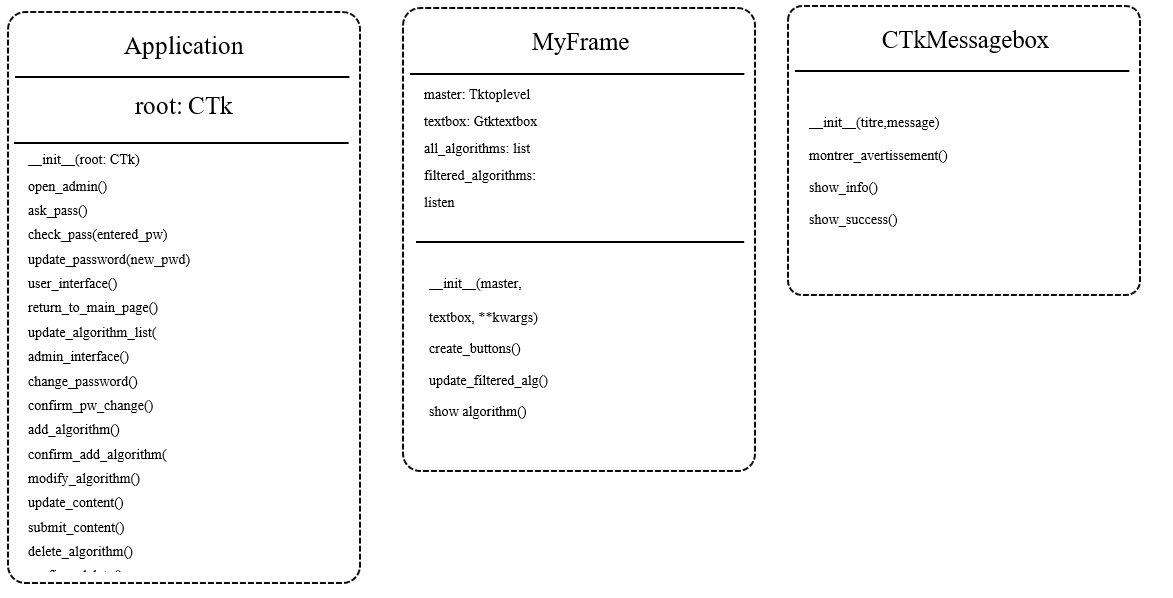
\includegraphics[width=0.9\linewidth]{images/classes}
	\caption{Диаграмма классов}
	\label{fig:classdiag}
\end{figure}



\ifПрактика{}\else{
	\section{Рабочий проект}
\subsection{Классы, используемые для разработки редактора}

Можно выделить следующий список классов и их методов, использованных при разработке web-приложения (таблица \ref{class:table}). Пример таблицы с уменьшенным межстрочным интервалом.

\renewcommand{\arraystretch}{0.9} % уменьшение расстояний до сетки таблицы
\begin{xltabular}{\textwidth}{|X|p{2.5cm}|>{\setlength{\baselineskip}{0.7\baselineskip}}p{4.85cm}|>{\setlength{\baselineskip}{0.7\baselineskip}}p{4.85cm}|}
	\caption{Описание классов, используемых в приложении\label{class:table}}\\
	\hline \centrow \setlength{\baselineskip}{0.7\baselineskip} Название класса & \centrow \setlength{\baselineskip}{0.7\baselineskip} Модуль, к которому относится класс & \centrow Описание класса & \centrow Методы \\
	\hline \centrow 1 & \centrow 2 & \centrow 3 & \centrow 4\\ \hline
	\endfirsthead
	\caption*{Продолжение таблицы \ref{class:table}}\\
	\hline \centrow 1 & \centrow 2 & \centrow 3 & \centrow 4\\ \hline
	\finishhead
	Application & app.py &  Этот класс представляет главное приложение ALGOLIB & \_init\_(root: CTk), open\_admin(),ask\_pass(), check\_pass(entered\_pw),	update\_password(), user\_interface(), return\_to\_main\_page() ,update\_algorithm\_list(), admin\_interface(), change\_password() ,confirm\_pw\_change(), add\_algorithm(), confirm\_add\_algorithm()
	,modify\_algorithm(), update\_content(), submit\_content(), delete\_algorithm().

	\hline  MyFrame & my\_frame.py & Этот класс представляет рамку, содержащую алгоритмы.  & \_init\_(master,textbox, **kwargs),	create\_buttons(), update\_filtered\_alg(), show algorithm(), master: Tktoplevel, textbox: Gtktextbox, all\_algorithms: list, filtered\_algorithms:, listen
	
	
	
	\hline CTk Messagebox & CTkMes- sageboxь & Этот класс представляет окно сообщения. Он отображает сообщения для пользователя. & Имеет дополнительные две точки для cross и init.
	
 \end{xltabular}
\renewcommand{\arraystretch}{1.0} % восстановление сетки



\subsection{Системное тестирование алгоритмической библиотеки .}
\begin{enumerate}
	
	\item Случай использования «алгоритм поиска»:
	\begin{itemize}
		\item основной исполнитель: пользователь;
		\item заинтересованные лица и их требования: пользователю необходимо добавить определенную фигуры на окно редактора;
		\item предусловие: пользователь открыл растровый редактор;
		\item ожидаемый результат: пользователь нажимает нужную горячую клавишу, ставит две координатные точки фигуры с помощью мышки, после этого фигура появляется на окно редактора. В итоге на окно редактора добавлятся выбранный пользователем геомерический обьект.
		\item результат представлен на рисунке 4.1
	\end{itemize}
	
	

	\begin{figure}[H]
		\centering
		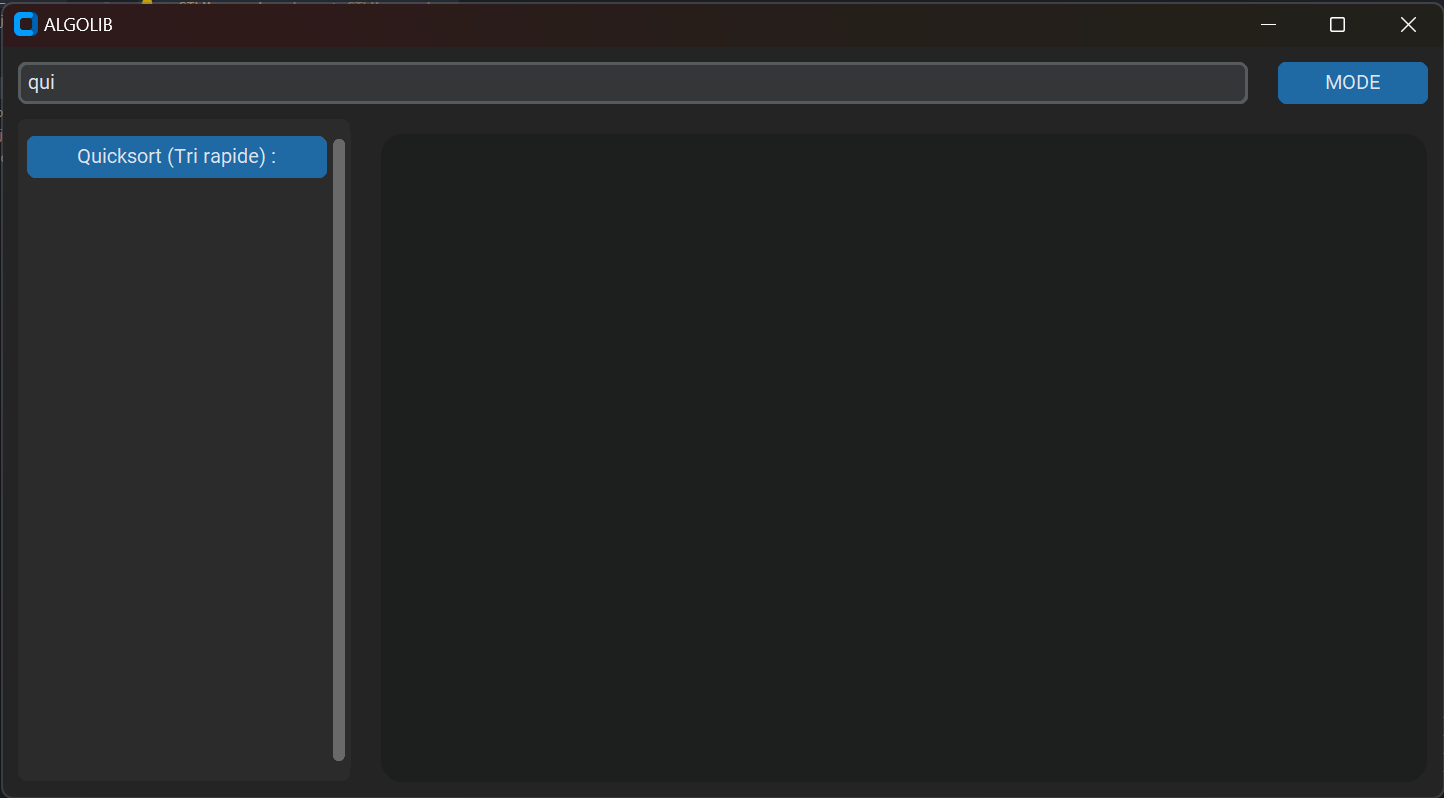
\includegraphics[width=0.7\linewidth]{images/adding}
		\caption{алгоритм поиска}
		\label{fig:classdiag}
	\end{figure}
	
	\item Случай использования «Удаление геометрического обьекта»:
	\begin{itemize}
		\item вариант использования "показать содержимое алгоритма"
		\item главный исполнитель: пользователь;
		\item заинтересованные стороны и их требования: пользователь нажимает кнопку в алгоритме, который он хочет;
		\item предварительное условие: пользователь открыл алгоритмическую библиотеку.
		\item ожидаемый результат: отображается описание географии.
			\item результат показан на рисунке 4.2.
	\end{itemize}
	
	\begin{figure}[H]
		\centering
		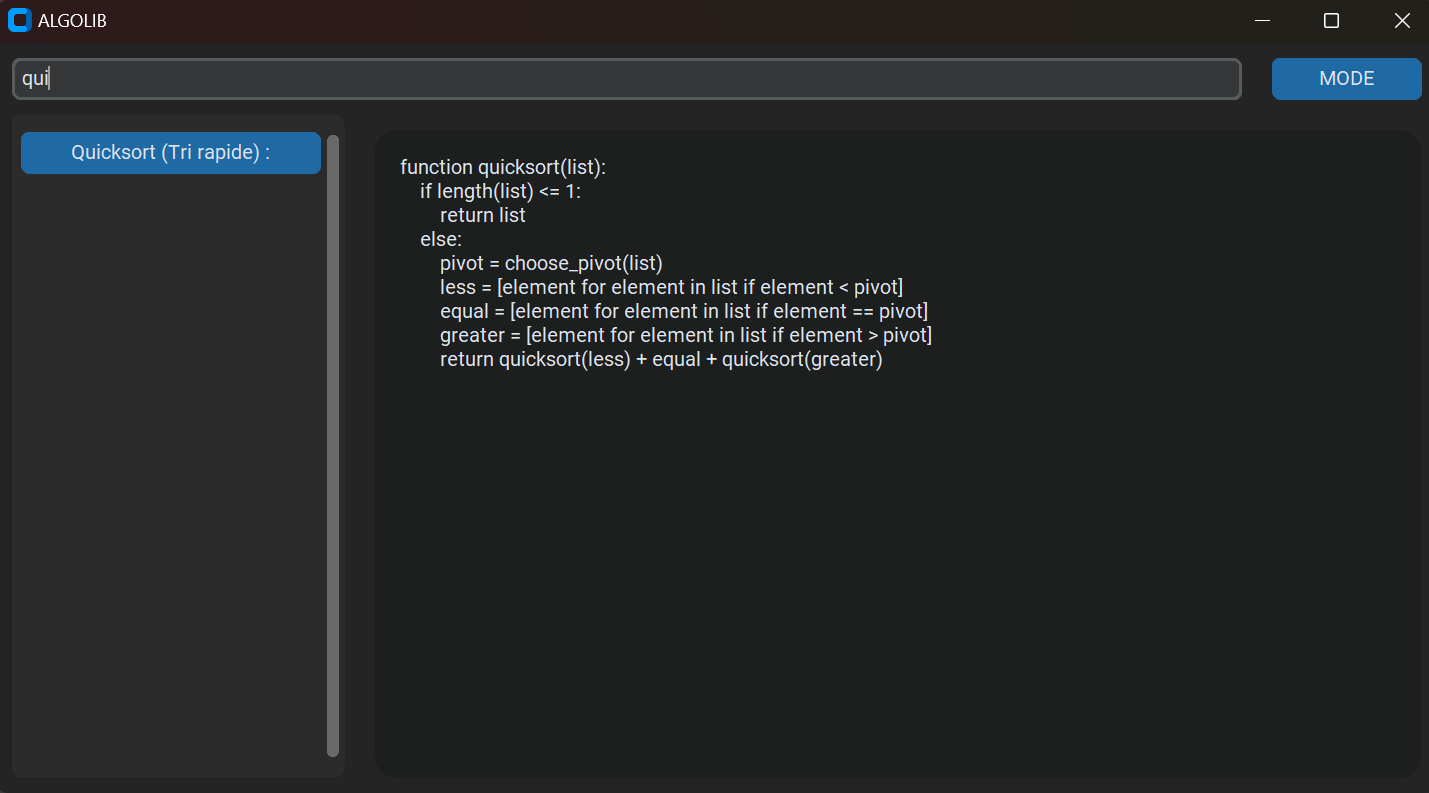
\includegraphics[width=0.7\linewidth]{images/delete}
		\caption{показан на рисунке }
		\label{fig:classdiag}
	\end{figure}
	
	
	
\end{enumerate}

	\section*{ЗАКЛЮЧЕНИЕ}
\addcontentsline{toc}{section}{ЗАКЛЮЧЕНИЕ}

Преимуществом алгоритмических библиотек является их гибкость, возможность быстрого поиска сложных алгоритмов.


Основные результаты работы:

\begin{enumerate}
	\item анализ предметной области. .
	\item была разработана концептуальная библиотечно-алгоритмическая модель. Разработайте модель системных данных. Системные требования определены.
	\item  была выполнена разработка алгоритмической библиотеки.
	\item  алгоритмическая библиотека была реализована и протестирована. Проведение
	калибровки.
	
\end{enumerate}

Все требования, объявленные в техническом задании, были полностью реализованы, все задачи, поставленные в начале разработки проекта, были также решены.

}\fi
\addcontentsline{toc}{section}{СПИСОК ИСПОЛЬЗОВАННЫХ ИСТОЧНИКОВ}

\begin{thebibliography}{99}
	
	\bibitem{freeman} Фримен, А. Практикум по программированию на Python / А. Фримен. – Москва : Вильямс, 2015. – 720 с. – ISBN 978-5-8459-1799-7.
	
	\bibitem{stroustrup} Страуструп, Б. Язык программирования C++. Лекции и упражнения / Б. Страуструп. – Санкт-Петербург : БХВ-Петербург, 2018. – 880 с. – ISBN 978-5-9579-2180-5.
	
	\bibitem{goodman} Гудман, Д. Полное руководство по разработке веб-приложений с использованием Django / Д. Гудман. – Москва : ДМК Пресс, 2017. – 624 с. – ISBN 978-5-94074-625-8.
	
	\bibitem{vanderplas} Вандер Плас, Дж. Python для сложных задач. Наука о данных и машинное обучение / Дж. Вандер Плас. – Санкт-Петербург : Питер, 2016. – 560 с. – ISBN 978-5-496-01049-8.
	
	\bibitem{lutz} Лутц, М. Изучаем Python. Программирование игр, визуализация данных, веб-приложения / М. Лутц. – Москва : ДМК Пресс, 2019. – 864 с. – ISBN 978-5-97060-729-5.
	
	\bibitem{tanenbaum} Таненбаум, Э. Архитектура компьютера / Э. Таненбаум. – Санкт-Петербург : Питер, 2014. – 896 с. – ISBN 978-5-496-01049-8.
	
	\bibitem{stallings} Сталлингс, У. Компьютерные сети. Принципы, технологии, протоколы / У. Сталлингс. – Москва : Издательский дом Вильямс, 2017. – 864 с. – ISBN 978-5-8459-2125-3.
	
	\bibitem{martin} Мартин, Р. Чистый код. Создание, анализ и рефакторинг / Р. Мартин. – Санкт-Петербург : Питер, 2018. – 464 с. – ISBN 978-5-4461-1089-3.
	
	\bibitem{kalender} Календер, Д. Принципы объектно-ориентированного программирования на С++ с примерами на C# и Java / Д. Календер. – Москва : ДМК Пресс, 2016. – 512 с. – ISBN 978-5-97060-858-2.
	
	\bibitem{hunter} Хантер, Э. Программирование на Python 3. Подробное руководство / Э. Хантер. – Москва : ДМК Пресс, 2019. – 560 с. – ISBN 978-5-97060-827-8.
	
\end{thebibliography}

\ifВКР{\appendix{Представление графического материала}

Графический материал, выполненный на отдельных листах,
изображен на рисунках А.1--А.\arabic{числоПлакатов}.
\setcounter{числоПлакатов}{0}

\renewcommand{\thefigure}{А.\arabic{figure}} % шаблон номера для плакатов

\begin{landscape}
	
	\begin{плакат}
		\includegraphics[width=0.82\linewidth]{плакат1.png}
		\заголовок{Сведения о ВКРБ}
		\label{pl1:image}      
	\end{плакат}
	
	\begin{плакат}
		\includegraphics[width=0.82\linewidth]{плакат2.png}
		\заголовок{Цель и задачи разработки}
		\label{pl2:image}      
	\end{плакат}
	
	\begin{плакат}
		\includegraphics[width=0.82\linewidth]{плакат3.png}
		\заголовок{Концептуальная модель сайта}
		\label{pl3:image}      
	\end{плакат}
	
	\begin{плакат}
		\includegraphics[width=0.82\linewidth]{плакат3.png}
		\заголовок{Еще плакат}
		\label{pl4:image}      
	\end{плакат}
	
\end{landscape}}\fi
\ifПрактика{}\else{\appendix{Фрагменты исходного кода программы}

\textbf{app.py}
\lstinputlisting[language=Python, frame=none]{app.py}

\textbf{my\_frame.py}
\lstinputlisting[language=Python, frame=none]{my_frame.py}
}\fi
\end{document}
